
% Default to the notebook output style




% Inherit from the specified cell style.





\documentclass{report}

% Default fixed font does not support bold face
\DeclareFixedFont{\ttb}{T1}{txtt}{bx}{n}{12} % for bold
\DeclareFixedFont{\ttm}{T1}{txtt}{m}{n}{12}  % for normal

% Custom colors
\usepackage{color}
\definecolor{deepblue}{rgb}{0,0,0.5}
\definecolor{deepred}{rgb}{0.6,0,0}
\definecolor{deepgreen}{rgb}{0,0.5,0}

\usepackage{listings}

% Python style for highlighting
\newcommand\pythonstyle{\lstset{
language=Python,
basicstyle=\ttm,
otherkeywords={self},             % Add keywords here
keywordstyle=\ttb\color{deepblue},
emph={MyClass,__init__},          % Custom highlighting
emphstyle=\ttb\color{deepred},    % Custom highlighting style
stringstyle=\color{deepgreen},
frame=tb,                         % Any extra options here
showstringspaces=false            %
}}


% Python environment
\lstnewenvironment{python}[1][]
{
\pythonstyle
\lstset{#1}
}
{}

    \usepackage[T1]{fontenc}
    % Nicer default font (+ math font) than Computer Modern for most use cases
    \usepackage{mathpazo}

    % Basic figure setup, for now with no caption control since it's done
    % automatically by Pandoc (which extracts ![](path) syntax from Markdown).
    \usepackage{graphicx}
    % We will generate all images so they have a width \maxwidth. This means
    % that they will get their normal width if they fit onto the page, but
    % are scaled down if they would overflow the margins.
    \makeatletter
    \def\maxwidth{\ifdim\Gin@nat@width>\linewidth\linewidth
    \else\Gin@nat@width\fi}
    \makeatother
    \let\Oldincludegraphics\includegraphics
    % Set max figure width to be 80% of text width, for now hardcoded.
    \renewcommand{\includegraphics}[1]{\Oldincludegraphics[width=.8\maxwidth]{#1}}
    % Ensure that by default, figures have no caption (until we provide a
    % proper Figure object with a Caption API and a way to capture that
    % in the conversion process - todo).
    \usepackage{caption}
    \DeclareCaptionLabelFormat{nolabel}{}
    \captionsetup{labelformat=nolabel}

    \usepackage{adjustbox} % Used to constrain images to a maximum size
    \usepackage{xcolor} % Allow colors to be defined
    \usepackage{enumerate} % Needed for markdown enumerations to work
    \usepackage{geometry} % Used to adjust the document margins
    \usepackage{amsmath} % Equations
    \usepackage{amssymb} % Equations
    \usepackage{textcomp} % defines textquotesingle
    % Hack from http://tex.stackexchange.com/a/47451/13684:
    \AtBeginDocument{%
        \def\PYZsq{\textquotesingle}% Upright quotes in Pygmentized code
    }
    \usepackage{upquote} % Upright quotes for verbatim code
    \usepackage{eurosym} % defines \euro
    \usepackage[mathletters]{ucs} % Extended unicode (utf-8) support
    \usepackage[utf8x]{inputenc} % Allow utf-8 characters in the tex document
    \usepackage{fancyvrb} % verbatim replacement that allows latex
    \usepackage{grffile} % extends the file name processing of package graphics
                         % to support a larger range
    % The hyperref package gives us a pdf with properly built
    % internal navigation ('pdf bookmarks' for the table of contents,
    % internal cross-reference links, web links for URLs, etc.)
    \usepackage{hyperref}
    \usepackage{longtable} % longtable support required by pandoc >1.10
    \usepackage{booktabs}  % table support for pandoc > 1.12.2
    \usepackage[inline]{enumitem} % IRkernel/repr support (it uses the enumerate* environment)
    \usepackage[normalem]{ulem} % ulem is needed to support strikethroughs (\sout)
                                % normalem makes italics be italics, not underlines




    % Colors for the hyperref package
    \definecolor{urlcolor}{rgb}{0,.145,.698}
    \definecolor{linkcolor}{rgb}{.71,0.21,0.01}
    \definecolor{citecolor}{rgb}{.12,.54,.11}

    % ANSI colors
    \definecolor{ansi-black}{HTML}{3E424D}
    \definecolor{ansi-black-intense}{HTML}{282C36}
    \definecolor{ansi-red}{HTML}{E75C58}
    \definecolor{ansi-red-intense}{HTML}{B22B31}
    \definecolor{ansi-green}{HTML}{00A250}
    \definecolor{ansi-green-intense}{HTML}{007427}
    \definecolor{ansi-yellow}{HTML}{DDB62B}
    \definecolor{ansi-yellow-intense}{HTML}{B27D12}
    \definecolor{ansi-blue}{HTML}{208FFB}
    \definecolor{ansi-blue-intense}{HTML}{0065CA}
    \definecolor{ansi-magenta}{HTML}{D160C4}
    \definecolor{ansi-magenta-intense}{HTML}{A03196}
    \definecolor{ansi-cyan}{HTML}{60C6C8}
    \definecolor{ansi-cyan-intense}{HTML}{258F8F}
    \definecolor{ansi-white}{HTML}{C5C1B4}
    \definecolor{ansi-white-intense}{HTML}{A1A6B2}

    % commands and environments needed by pandoc snippets
    % extracted from the output of `pandoc -s`
    \providecommand{\tightlist}{%
      \setlength{\itemsep}{0pt}\setlength{\parskip}{0pt}}
    \DefineVerbatimEnvironment{Highlighting}{Verbatim}{commandchars=\\\{\}}
    % Add ',fontsize=\small' for more characters per line
    \newenvironment{Shaded}{}{}
    \newcommand{\KeywordTok}[1]{\textcolor[rgb]{0.00,0.44,0.13}{\textbf{{#1}}}}
    \newcommand{\DataTypeTok}[1]{\textcolor[rgb]{0.56,0.13,0.00}{{#1}}}
    \newcommand{\DecValTok}[1]{\textcolor[rgb]{0.25,0.63,0.44}{{#1}}}
    \newcommand{\BaseNTok}[1]{\textcolor[rgb]{0.25,0.63,0.44}{{#1}}}
    \newcommand{\FloatTok}[1]{\textcolor[rgb]{0.25,0.63,0.44}{{#1}}}
    \newcommand{\CharTok}[1]{\textcolor[rgb]{0.25,0.44,0.63}{{#1}}}
    \newcommand{\StringTok}[1]{\textcolor[rgb]{0.25,0.44,0.63}{{#1}}}
    \newcommand{\CommentTok}[1]{\textcolor[rgb]{0.38,0.63,0.69}{\textit{{#1}}}}
    \newcommand{\OtherTok}[1]{\textcolor[rgb]{0.00,0.44,0.13}{{#1}}}
    \newcommand{\AlertTok}[1]{\textcolor[rgb]{1.00,0.00,0.00}{\textbf{{#1}}}}
    \newcommand{\FunctionTok}[1]{\textcolor[rgb]{0.02,0.16,0.49}{{#1}}}
    \newcommand{\RegionMarkerTok}[1]{{#1}}
    \newcommand{\ErrorTok}[1]{\textcolor[rgb]{1.00,0.00,0.00}{\textbf{{#1}}}}
    \newcommand{\NormalTok}[1]{{#1}}

    % Additional commands for more recent versions of Pandoc
    \newcommand{\ConstantTok}[1]{\textcolor[rgb]{0.53,0.00,0.00}{{#1}}}
    \newcommand{\SpecialCharTok}[1]{\textcolor[rgb]{0.25,0.44,0.63}{{#1}}}
    \newcommand{\VerbatimStringTok}[1]{\textcolor[rgb]{0.25,0.44,0.63}{{#1}}}
    \newcommand{\SpecialStringTok}[1]{\textcolor[rgb]{0.73,0.40,0.53}{{#1}}}
    \newcommand{\ImportTok}[1]{{#1}}
    \newcommand{\DocumentationTok}[1]{\textcolor[rgb]{0.73,0.13,0.13}{\textit{{#1}}}}
    \newcommand{\AnnotationTok}[1]{\textcolor[rgb]{0.38,0.63,0.69}{\textbf{\textit{{#1}}}}}
    \newcommand{\CommentVarTok}[1]{\textcolor[rgb]{0.38,0.63,0.69}{\textbf{\textit{{#1}}}}}
    \newcommand{\VariableTok}[1]{\textcolor[rgb]{0.10,0.09,0.49}{{#1}}}
    \newcommand{\ControlFlowTok}[1]{\textcolor[rgb]{0.00,0.44,0.13}{\textbf{{#1}}}}
    \newcommand{\OperatorTok}[1]{\textcolor[rgb]{0.40,0.40,0.40}{{#1}}}
    \newcommand{\BuiltInTok}[1]{{#1}}
    \newcommand{\ExtensionTok}[1]{{#1}}
    \newcommand{\PreprocessorTok}[1]{\textcolor[rgb]{0.74,0.48,0.00}{{#1}}}
    \newcommand{\AttributeTok}[1]{\textcolor[rgb]{0.49,0.56,0.16}{{#1}}}
    \newcommand{\InformationTok}[1]{\textcolor[rgb]{0.38,0.63,0.69}{\textbf{\textit{{#1}}}}}
    \newcommand{\WarningTok}[1]{\textcolor[rgb]{0.38,0.63,0.69}{\textbf{\textit{{#1}}}}}


    % Define a nice break command that doesn't care if a line doesn't already
    % exist.
    \def\br{\hspace*{\fill} \\* }
    % Math Jax compatability definitions
    \def\gt{>}
    \def\lt{<}
    % Document parameters
    \title{Neuromorphic\_Silicon\_Photonics}




    % Pygments definitions

\makeatletter
\def\PY@reset{\let\PY@it=\relax \let\PY@bf=\relax%
    \let\PY@ul=\relax \let\PY@tc=\relax%
    \let\PY@bc=\relax \let\PY@ff=\relax}
\def\PY@tok#1{\csname PY@tok@#1\endcsname}
\def\PY@toks#1+{\ifx\relax#1\empty\else%
    \PY@tok{#1}\expandafter\PY@toks\fi}
\def\PY@do#1{\PY@bc{\PY@tc{\PY@ul{%
    \PY@it{\PY@bf{\PY@ff{#1}}}}}}}
\def\PY#1#2{\PY@reset\PY@toks#1+\relax+\PY@do{#2}}

\expandafter\def\csname PY@tok@w\endcsname{\def\PY@tc##1{\textcolor[rgb]{0.73,0.73,0.73}{##1}}}
\expandafter\def\csname PY@tok@c\endcsname{\let\PY@it=\textit\def\PY@tc##1{\textcolor[rgb]{0.25,0.50,0.50}{##1}}}
\expandafter\def\csname PY@tok@cp\endcsname{\def\PY@tc##1{\textcolor[rgb]{0.74,0.48,0.00}{##1}}}
\expandafter\def\csname PY@tok@k\endcsname{\let\PY@bf=\textbf\def\PY@tc##1{\textcolor[rgb]{0.00,0.50,0.00}{##1}}}
\expandafter\def\csname PY@tok@kp\endcsname{\def\PY@tc##1{\textcolor[rgb]{0.00,0.50,0.00}{##1}}}
\expandafter\def\csname PY@tok@kt\endcsname{\def\PY@tc##1{\textcolor[rgb]{0.69,0.00,0.25}{##1}}}
\expandafter\def\csname PY@tok@o\endcsname{\def\PY@tc##1{\textcolor[rgb]{0.40,0.40,0.40}{##1}}}
\expandafter\def\csname PY@tok@ow\endcsname{\let\PY@bf=\textbf\def\PY@tc##1{\textcolor[rgb]{0.67,0.13,1.00}{##1}}}
\expandafter\def\csname PY@tok@nb\endcsname{\def\PY@tc##1{\textcolor[rgb]{0.00,0.50,0.00}{##1}}}
\expandafter\def\csname PY@tok@nf\endcsname{\def\PY@tc##1{\textcolor[rgb]{0.00,0.00,1.00}{##1}}}
\expandafter\def\csname PY@tok@nc\endcsname{\let\PY@bf=\textbf\def\PY@tc##1{\textcolor[rgb]{0.00,0.00,1.00}{##1}}}
\expandafter\def\csname PY@tok@nn\endcsname{\let\PY@bf=\textbf\def\PY@tc##1{\textcolor[rgb]{0.00,0.00,1.00}{##1}}}
\expandafter\def\csname PY@tok@ne\endcsname{\let\PY@bf=\textbf\def\PY@tc##1{\textcolor[rgb]{0.82,0.25,0.23}{##1}}}
\expandafter\def\csname PY@tok@nv\endcsname{\def\PY@tc##1{\textcolor[rgb]{0.10,0.09,0.49}{##1}}}
\expandafter\def\csname PY@tok@no\endcsname{\def\PY@tc##1{\textcolor[rgb]{0.53,0.00,0.00}{##1}}}
\expandafter\def\csname PY@tok@nl\endcsname{\def\PY@tc##1{\textcolor[rgb]{0.63,0.63,0.00}{##1}}}
\expandafter\def\csname PY@tok@ni\endcsname{\let\PY@bf=\textbf\def\PY@tc##1{\textcolor[rgb]{0.60,0.60,0.60}{##1}}}
\expandafter\def\csname PY@tok@na\endcsname{\def\PY@tc##1{\textcolor[rgb]{0.49,0.56,0.16}{##1}}}
\expandafter\def\csname PY@tok@nt\endcsname{\let\PY@bf=\textbf\def\PY@tc##1{\textcolor[rgb]{0.00,0.50,0.00}{##1}}}
\expandafter\def\csname PY@tok@nd\endcsname{\def\PY@tc##1{\textcolor[rgb]{0.67,0.13,1.00}{##1}}}
\expandafter\def\csname PY@tok@s\endcsname{\def\PY@tc##1{\textcolor[rgb]{0.73,0.13,0.13}{##1}}}
\expandafter\def\csname PY@tok@sd\endcsname{\let\PY@it=\textit\def\PY@tc##1{\textcolor[rgb]{0.73,0.13,0.13}{##1}}}
\expandafter\def\csname PY@tok@si\endcsname{\let\PY@bf=\textbf\def\PY@tc##1{\textcolor[rgb]{0.73,0.40,0.53}{##1}}}
\expandafter\def\csname PY@tok@se\endcsname{\let\PY@bf=\textbf\def\PY@tc##1{\textcolor[rgb]{0.73,0.40,0.13}{##1}}}
\expandafter\def\csname PY@tok@sr\endcsname{\def\PY@tc##1{\textcolor[rgb]{0.73,0.40,0.53}{##1}}}
\expandafter\def\csname PY@tok@ss\endcsname{\def\PY@tc##1{\textcolor[rgb]{0.10,0.09,0.49}{##1}}}
\expandafter\def\csname PY@tok@sx\endcsname{\def\PY@tc##1{\textcolor[rgb]{0.00,0.50,0.00}{##1}}}
\expandafter\def\csname PY@tok@m\endcsname{\def\PY@tc##1{\textcolor[rgb]{0.40,0.40,0.40}{##1}}}
\expandafter\def\csname PY@tok@gh\endcsname{\let\PY@bf=\textbf\def\PY@tc##1{\textcolor[rgb]{0.00,0.00,0.50}{##1}}}
\expandafter\def\csname PY@tok@gu\endcsname{\let\PY@bf=\textbf\def\PY@tc##1{\textcolor[rgb]{0.50,0.00,0.50}{##1}}}
\expandafter\def\csname PY@tok@gd\endcsname{\def\PY@tc##1{\textcolor[rgb]{0.63,0.00,0.00}{##1}}}
\expandafter\def\csname PY@tok@gi\endcsname{\def\PY@tc##1{\textcolor[rgb]{0.00,0.63,0.00}{##1}}}
\expandafter\def\csname PY@tok@gr\endcsname{\def\PY@tc##1{\textcolor[rgb]{1.00,0.00,0.00}{##1}}}
\expandafter\def\csname PY@tok@ge\endcsname{\let\PY@it=\textit}
\expandafter\def\csname PY@tok@gs\endcsname{\let\PY@bf=\textbf}
\expandafter\def\csname PY@tok@gp\endcsname{\let\PY@bf=\textbf\def\PY@tc##1{\textcolor[rgb]{0.00,0.00,0.50}{##1}}}
\expandafter\def\csname PY@tok@go\endcsname{\def\PY@tc##1{\textcolor[rgb]{0.53,0.53,0.53}{##1}}}
\expandafter\def\csname PY@tok@gt\endcsname{\def\PY@tc##1{\textcolor[rgb]{0.00,0.27,0.87}{##1}}}
\expandafter\def\csname PY@tok@err\endcsname{\def\PY@bc##1{\setlength{\fboxsep}{0pt}\fcolorbox[rgb]{1.00,0.00,0.00}{1,1,1}{\strut ##1}}}
\expandafter\def\csname PY@tok@kc\endcsname{\let\PY@bf=\textbf\def\PY@tc##1{\textcolor[rgb]{0.00,0.50,0.00}{##1}}}
\expandafter\def\csname PY@tok@kd\endcsname{\let\PY@bf=\textbf\def\PY@tc##1{\textcolor[rgb]{0.00,0.50,0.00}{##1}}}
\expandafter\def\csname PY@tok@kn\endcsname{\let\PY@bf=\textbf\def\PY@tc##1{\textcolor[rgb]{0.00,0.50,0.00}{##1}}}
\expandafter\def\csname PY@tok@kr\endcsname{\let\PY@bf=\textbf\def\PY@tc##1{\textcolor[rgb]{0.00,0.50,0.00}{##1}}}
\expandafter\def\csname PY@tok@bp\endcsname{\def\PY@tc##1{\textcolor[rgb]{0.00,0.50,0.00}{##1}}}
\expandafter\def\csname PY@tok@fm\endcsname{\def\PY@tc##1{\textcolor[rgb]{0.00,0.00,1.00}{##1}}}
\expandafter\def\csname PY@tok@vc\endcsname{\def\PY@tc##1{\textcolor[rgb]{0.10,0.09,0.49}{##1}}}
\expandafter\def\csname PY@tok@vg\endcsname{\def\PY@tc##1{\textcolor[rgb]{0.10,0.09,0.49}{##1}}}
\expandafter\def\csname PY@tok@vi\endcsname{\def\PY@tc##1{\textcolor[rgb]{0.10,0.09,0.49}{##1}}}
\expandafter\def\csname PY@tok@vm\endcsname{\def\PY@tc##1{\textcolor[rgb]{0.10,0.09,0.49}{##1}}}
\expandafter\def\csname PY@tok@sa\endcsname{\def\PY@tc##1{\textcolor[rgb]{0.73,0.13,0.13}{##1}}}
\expandafter\def\csname PY@tok@sb\endcsname{\def\PY@tc##1{\textcolor[rgb]{0.73,0.13,0.13}{##1}}}
\expandafter\def\csname PY@tok@sc\endcsname{\def\PY@tc##1{\textcolor[rgb]{0.73,0.13,0.13}{##1}}}
\expandafter\def\csname PY@tok@dl\endcsname{\def\PY@tc##1{\textcolor[rgb]{0.73,0.13,0.13}{##1}}}
\expandafter\def\csname PY@tok@s2\endcsname{\def\PY@tc##1{\textcolor[rgb]{0.73,0.13,0.13}{##1}}}
\expandafter\def\csname PY@tok@sh\endcsname{\def\PY@tc##1{\textcolor[rgb]{0.73,0.13,0.13}{##1}}}
\expandafter\def\csname PY@tok@s1\endcsname{\def\PY@tc##1{\textcolor[rgb]{0.73,0.13,0.13}{##1}}}
\expandafter\def\csname PY@tok@mb\endcsname{\def\PY@tc##1{\textcolor[rgb]{0.40,0.40,0.40}{##1}}}
\expandafter\def\csname PY@tok@mf\endcsname{\def\PY@tc##1{\textcolor[rgb]{0.40,0.40,0.40}{##1}}}
\expandafter\def\csname PY@tok@mh\endcsname{\def\PY@tc##1{\textcolor[rgb]{0.40,0.40,0.40}{##1}}}
\expandafter\def\csname PY@tok@mi\endcsname{\def\PY@tc##1{\textcolor[rgb]{0.40,0.40,0.40}{##1}}}
\expandafter\def\csname PY@tok@il\endcsname{\def\PY@tc##1{\textcolor[rgb]{0.40,0.40,0.40}{##1}}}
\expandafter\def\csname PY@tok@mo\endcsname{\def\PY@tc##1{\textcolor[rgb]{0.40,0.40,0.40}{##1}}}
\expandafter\def\csname PY@tok@ch\endcsname{\let\PY@it=\textit\def\PY@tc##1{\textcolor[rgb]{0.25,0.50,0.50}{##1}}}
\expandafter\def\csname PY@tok@cm\endcsname{\let\PY@it=\textit\def\PY@tc##1{\textcolor[rgb]{0.25,0.50,0.50}{##1}}}
\expandafter\def\csname PY@tok@cpf\endcsname{\let\PY@it=\textit\def\PY@tc##1{\textcolor[rgb]{0.25,0.50,0.50}{##1}}}
\expandafter\def\csname PY@tok@c1\endcsname{\let\PY@it=\textit\def\PY@tc##1{\textcolor[rgb]{0.25,0.50,0.50}{##1}}}
\expandafter\def\csname PY@tok@cs\endcsname{\let\PY@it=\textit\def\PY@tc##1{\textcolor[rgb]{0.25,0.50,0.50}{##1}}}

\def\PYZbs{\char`\\}
\def\PYZus{\char`\_}
\def\PYZob{\char`\{}
\def\PYZcb{\char`\}}
\def\PYZca{\char`\^}
\def\PYZam{\char`\&}
\def\PYZlt{\char`\<}
\def\PYZgt{\char`\>}
\def\PYZsh{\char`\#}
\def\PYZpc{\char`\%}
\def\PYZdl{\char`\$}
\def\PYZhy{\char`\-}
\def\PYZsq{\char`\'}
\def\PYZdq{\char`\"}
\def\PYZti{\char`\~}
% for compatibility with earlier versions
\def\PYZat{@}
\def\PYZlb{[}
\def\PYZrb{]}
\makeatother


    % Exact colors from NB
    \definecolor{incolor}{rgb}{0.0, 0.0, 0.5}
    \definecolor{outcolor}{rgb}{0.545, 0.0, 0.0}




    % Prevent overflowing lines due to hard-to-break entities
    \sloppy
    % Setup hyperref package
    \hypersetup{
      breaklinks=true,  % so long urls are correctly broken across lines
      colorlinks=true,
      urlcolor=urlcolor,
      linkcolor=linkcolor,
      citecolor=citecolor,
      }
    % Slightly bigger margins than the latex defaults

    \geometry{verbose,tmargin=1in,bmargin=1in,lmargin=1in,rmargin=1in}



    \begin{document}



    \maketitle


    \tableofcontents



\chapter{Solving ODEs with Photonic Modulator
Neurons}\label{solving-odes-with-photonic-modulator-neurons}

This notebook was created to support the publication of an article
titled \href{https://arxiv.org/abs/1611.02272}{\emph{Neuromorphic
Silicon Photonics}}, authored by Alexander N. Tait, Ellen Zhou, Thomas
Ferreira de Lima, Allie X. Wu, Mitchell A. Nahmias, Bhavin J. Shastri
and Paul R. Prucnal, first submitted on 5 Nov 2016.

A copy of this notebook is available at:

https://github.com/lightwave-lab/Neuromorphic\_Silicon\_Photonics


\section{Modifications to the nengo
project}\label{modifications-to-the-nengo-project}

Nengo is based exclusively on monotonic, non-negative output neuron
models. However, its encoding-decoding algorithms should work with other
kinds of neuron models. Here, we use the following
\texttt{FourierSinusoid} class of neurons included in our fork of the
\href{https://github.com/nengo/nengo/}{nengo project}.


\section{The Lorenz chaotic
attractor}\label{the-lorenz-chaotic-attractor}

In this simulation, we chose to construct a neural network using the
neurons defined \protect\hyperlink{fourier_neuron_nengo}{above} to solve
a classical chaotic dynamical system named ``Lorenz attractor''.

The equations are:

\[
\dot{x}_0 = \nu(x_1 - x_0) \\
\dot{x}_1 = x_0 (\rho - x_2) - x_1  \\
\dot{x}_2 = x_0 x_1 - \beta x_2
\]

Since \(x_2\) is centered around approximately \(\rho\), and since NEF
ensembles are usually optimized to represent values within a certain
radius of the origin, we substitute \(x_2' = x_2 - \rho\), giving these
equations: \[
\dot{x}_0 = \nu(x_1 - x_0) \\
\dot{x}_1 = - x_0 x_2' - x_1\\
\dot{x}_2' = x_0 x_1 - \beta (x_2' + \rho)
\]

Refer to the standard example of the Lorenz attractor solver with 2000
neurons in a
\href{https://github.com/nengo/nengo/blob/master/examples/dynamics/lorenz_attractor.ipynb}{nengo
example}. *Note that the last equation for \(x_2'\) is typically shown
with an error in that example and in other articles from
Prof.~Eliasmith's group.

\section{Encoding strategy}\label{encoding-strategy}

From here onwards, we will refer the Lorenz system in its reduced form
as as \(\vec x = f(\vec x)\), with:

\[
\vec x = [x_0, x_1, x_2']^T
\]

and

\[
f(\vec x) = \left[
\begin{array}{c}
\nu(x_1 - x_0) \\
- x_0 x_2'- x_1 \\
x_0 x_1 - \beta (x_2' + \rho)
\end{array}
\right]
\]

This is specified to nengo like this...
\begin{python}
# the ODE to emulate
# The default values for sigma, beta and rho originally used by Lorenz.
# Cf. https://en.wikipedia.org/wiki/Lorenz_system#Analysis
nu = 10
beta = 8.0/3
rho = 28
def feedback(x):
    dx0 = (-nu * x[0] + nu * x[1]) / gamma
    dx1 = (-x[0] * x[2] - x[1]) / gamma
    dx2 = (x[0] * x[1] - beta * (x[2] + rho)) / gamma

    return [dx0 * tau + x[0],
            dx1 * tau + x[1],
            dx2 * tau + x[2]]
\end{python}

Hooking it up:
\begin{python}
# The main ensemble
state = nengo.Ensemble(num_neurons, dimensions=3,
    intercepts=intercepts,
    neuron_type=nengo.neurons.FourierSinusoid(max_overall_rate=max_transmission,
                                              s_pi=s_pi),
    max_rates=max_rates,
    encoders=encoders, radius=60.)

# This special node calls a function every timestep,
# in this case a class method of delay
delay_node = nengo.Node(delay.step, size_in=3, size_out=3)

# Connections from state to delay and back
cdel = nengo.Connection(state, delay_node,
                        function=feedback, synapse=tau)
conn = nengo.Connection(delay_node, state)
\end{python}

\subsection{Neuron model}\label{neuron-model}

Using \href{http://www.nengo.ca}{nengo}, we instantiate a population of
\(N\) neurons that are all-to-all interconnected. These neurons are
responsible of \emph{representing} the vector \(\vec x\) at any time
\(t\). We consider the state of each neuron as \(\vec s = [s_i]\) for
neuron \(i\). The ODE that models each neuron, in this case, is:

\[\tau s_i + s_i = u_i \] where \(u_i\) represents the post-synaptic
input of the neuron and \(y_i=\sigma(s_i)\) its output.

\subsection{Nengo encoding strategy}\label{nengo-encoding-strategy}

In order to \emph{encode} a vector \(\vec x\) in the population \(N\),
nengo performs the following linear transformation (it has to be linear
for the method to work):

\[ s_i = g_i \vec e_i \cdot \vec x + b_i \] where \(g_i\) is a gain
term, \(\vec e_i\) is an encoder vector, and \(b_i\) is a bias term.
This is called the \emph{encoding strategy}.

Nonlinear operations are effectively performed by linear combinations of
the neural nonlinearities \(\sigma(s_i)\). Therefore, it is the
encoder's mission to generate as much entropy about the variables
\(\vec x\) as possible. This can be done by generating a diverse set of
\((g, \vec e, b)\) parameters. Below, we do this by using
\(\vec e_i = [1, \pm 1, \pm1]\), mixing all components of \(\vec x\)
together. Note: this can be optimized even further by noticing that the
ODE does not contain \(x_0 x_2\) terms.

Because we know that \(\sigma\) is a sinusoid, we create a set of
\((g,b)\) values to span a Fourier-like basis of functions across the
domain \(\vec e_i \cdot \vec x \in [-1,1]\). (See
\protect\hyperlink{tuning_curves}{tuning curves}).

\begin{python}
# Intercept, in this case, corresponds to where the tuning curve intercepts
# zero. Range of [-.5, .5] corresponds to [-pi, pi]
ints = [0, 1/4]
# This number represents how many periods do we want between -1 and 1
# (see tuning curves below)
rats = s_pi * np.arange(1, 4)/2
# Encoder multipliers
enst = [-1,1]

num_intercepts = len(ints)
num_max_rates = len(rats)
num_encoders = len(enst) ** 2

j = 0
encoders = np.zeros(shape=(num_neurons, 3))
intercepts = np.zeros(num_neurons)
max_rates = np.zeros_like(intercepts)
for ir in range(num_max_rates):
    for ii in range(num_intercepts):
        for ie0 in range(len(enst)):
            if ie0 is 0:
                continue
            for ie1 in range(len(enst)):
                for ie2 in range(len(enst)):
                    vertex = np.array([enst[ie0], enst[ie1], enst[ie2]])
                    if not np.all(vertex == 0):
                        encoders[j,:] = vertex
                        intercepts[j] = ints[ii]
                        max_rates[j] = rats[ir]
                        j += 1
\end{python}

\subsection{Timing}
\begin{python}
# Round-trip feedback delay in ns
delayTime = .048
# gamma is a characteristic time scale in real time units
# The coefficient gamma/delayTime determines the stability
# In paper, coefficient was 65 (spurious), 104 (inaccurate), 260 (looks good)
gamma = 260 * delayTime

# We'll make a simple object to implement the delayed feedback
class Delay(object):
    def __init__(self, dimensions, timesteps=50):
        timesteps = max(timesteps,1)
        self.history = np.zeros((timesteps, dimensions))
    def step(self, t, x):
        self.history = np.roll(self.history, -1, axis=0)
        self.history[-1] = x
        return self.history[0]
delay = Delay(3, timesteps=int(delayTime / dt))
\end{python}


\subsection{Tuning curves in Fourier
basis}\label{tuning-curves-in-fourier-basis}

Here, assuming that the neuron states are
\(s_i = g_i \vec e_i \cdot \vec x + b_i\), we plot the functions
\(\sigma(s_i)\) for neurons with different \(g_i, b_i\) values according
to the previous \protect\hyperlink{Encoding-strategy}{table}.

    \begin{center}
    \adjustimage{max size={0.9\linewidth}{0.9\paperheight}}{Neuromorphic_Silicon_Photonics_files/Neuromorphic_Silicon_Photonics_7_0.png}
    \end{center}
    { \hspace*{\fill} \\}

\section{Decoding strategy: calculating weight
matrix}\label{decoding-strategy-calculating-weight-matrix}

\begin{figure}
\centering
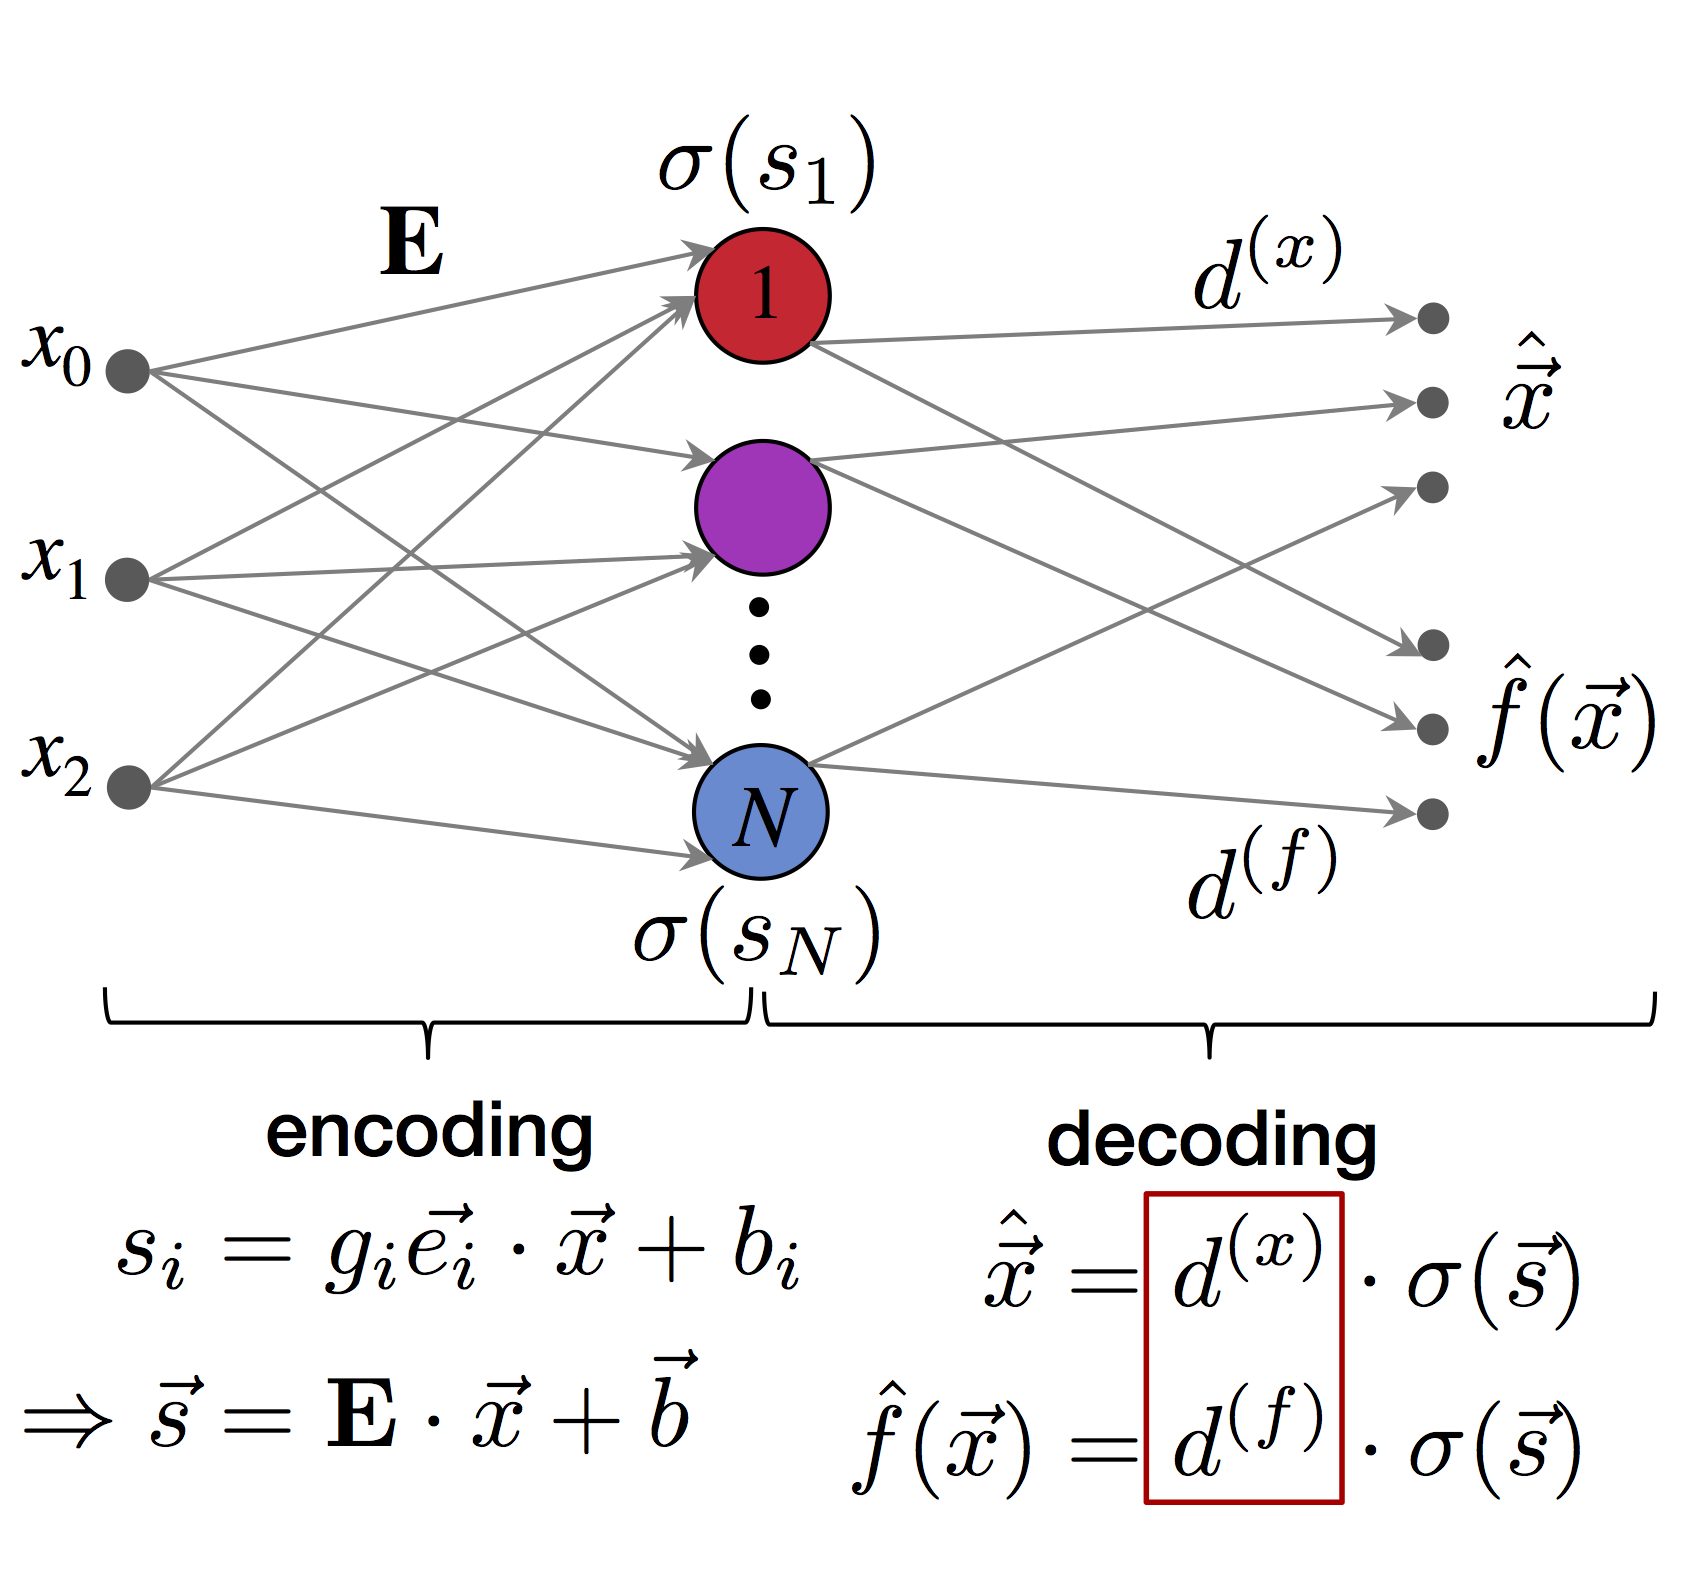
\includegraphics{Fig1.png}
\caption{}
\end{figure}

As mentioned, nengo decodes a function \(h(\vec x)\) from the population
of neurons by a linear decoding strategy, i.e.~a matrix \(d^{(h)}\)
resulting in an estimator \(\hat h(\vec x)\):

\[\hat h(\vec x) = d^{(h)} \vec y\] where
\(y_i = \sigma(s_i) = \sigma(g_i \vec e_i \cdot \vec x + b_i)\\\).

This matrix \(d^{(h)}\) is uniquely dependent on the encoder strategy,
the neuron's transfer function \(\sigma\) and the function \(h\). As a
result, it can be pre-computed before any real-time simulation. Namely,
it attempts to minimize the following objective function:

\[J = \int \left\lVert d^{(h)}\vec y - h(\vec x)\right\rVert \mathrm{d}\vec x\]
where the integral is over the desired range of values of \(\vec x\).

The minimum can be calculated via the Moore-Penrose pseudoinverse method
(\href{https://doi.org/10.3389/neuro.11.007.2009}{Stewart et al. Front
Neuroinform. 3 (2009)}):

\[
\Gamma_{ij} = \int y_i y_j \mathrm{d}\vec x
\] \[
\Upsilon_i = \int y_i h(\vec x) \mathrm{d} \vec x
\] \[
d^{(h)} = \Gamma^{-1} \cdot \Upsilon
\]

\subsection{Weight matrix}\label{weight-matrix}

\begin{figure}
\centering
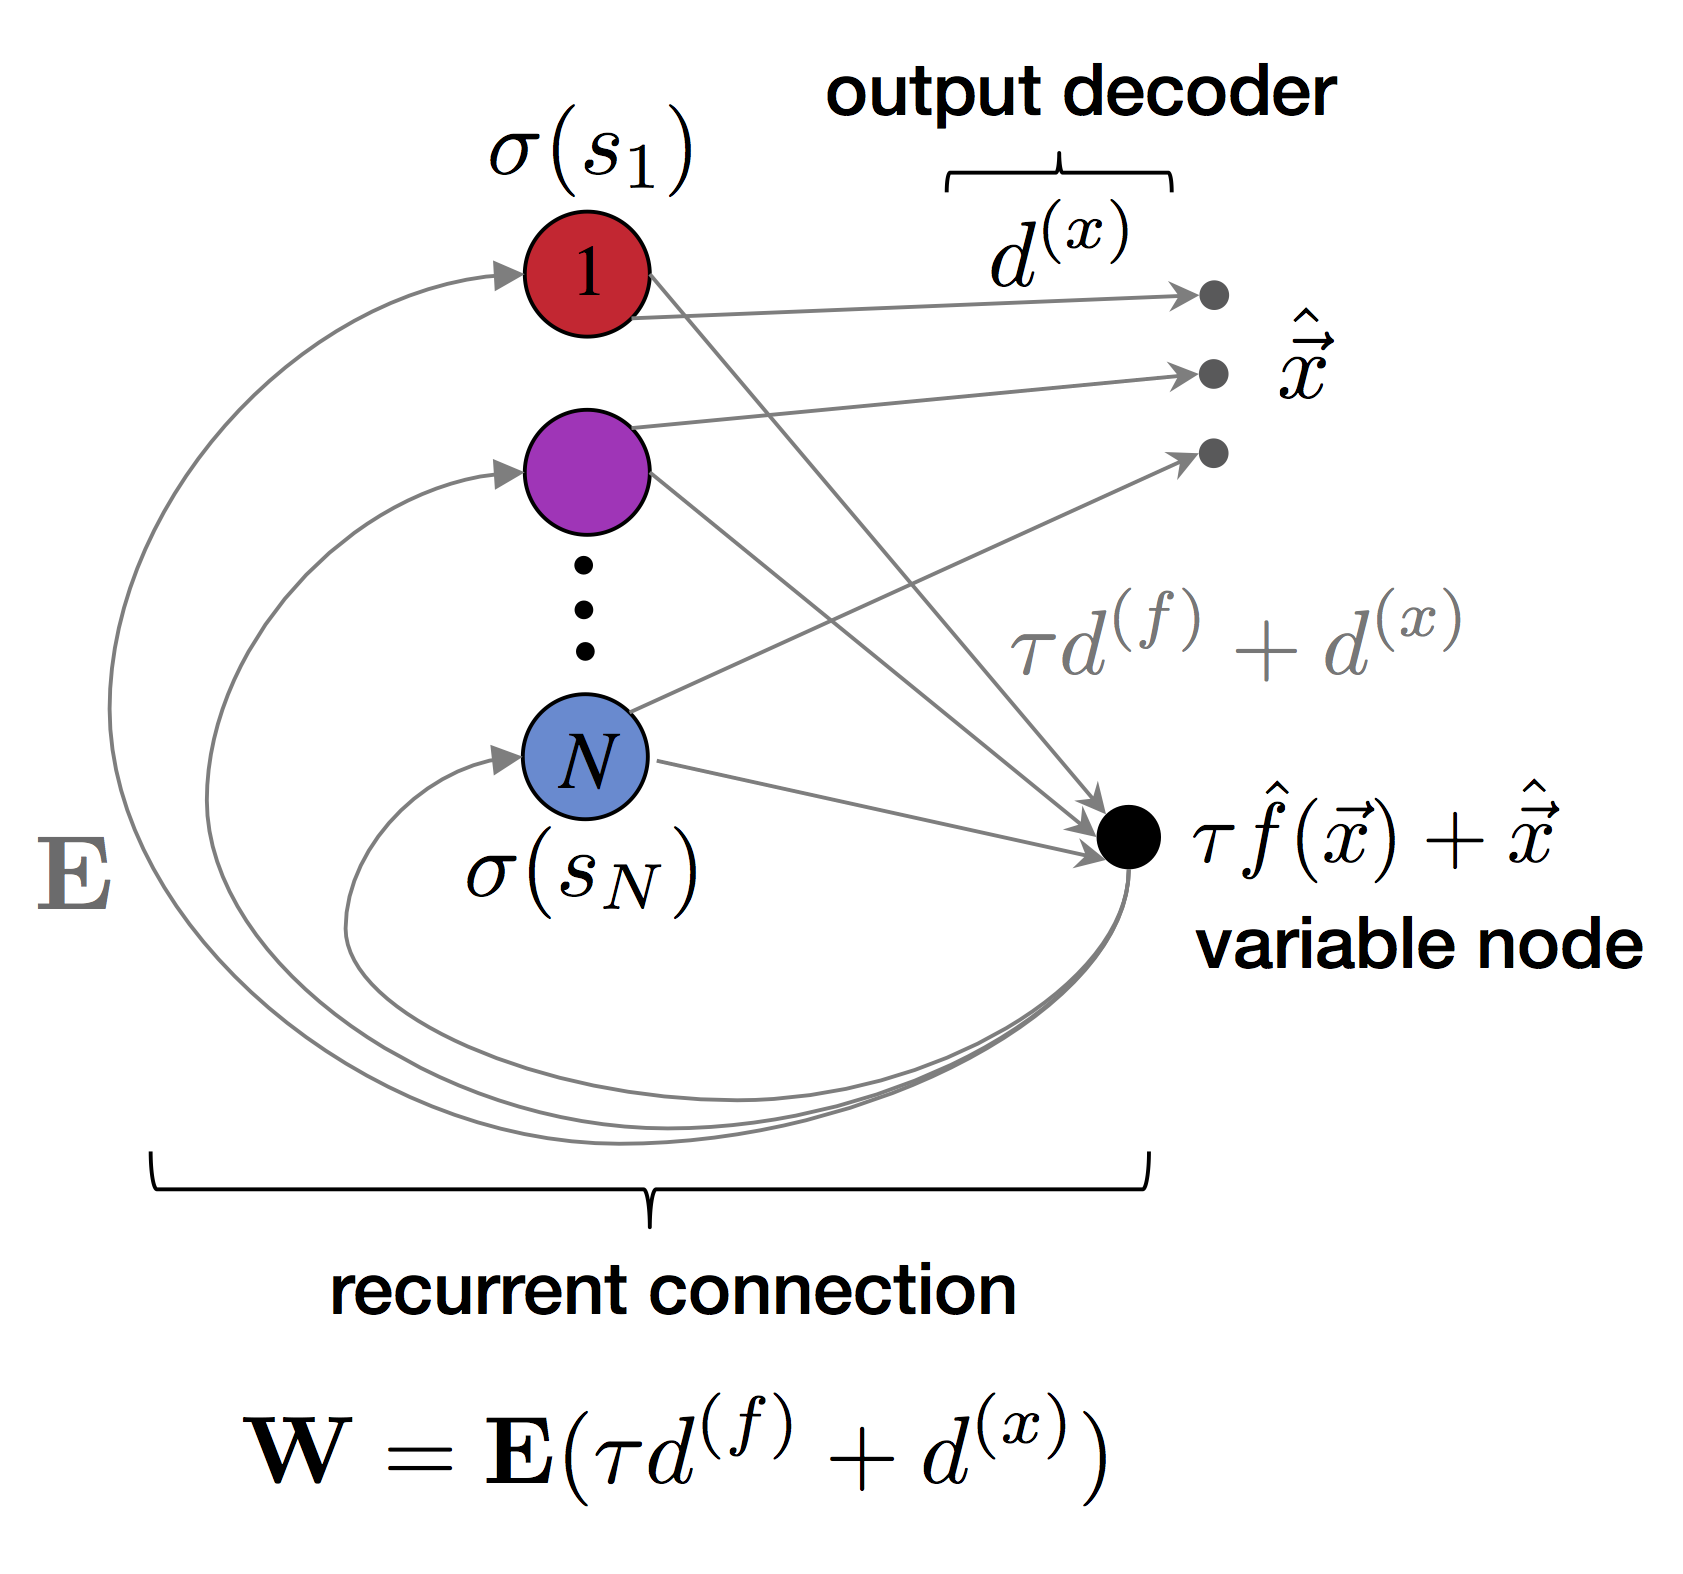
\includegraphics{Fig2.png}
\caption{}
\end{figure}

If we add an all-to-all recurrent connection to the neural population,
their collective dynamics is described by the following ODE system:

\[ \tau  \dot{\vec s} + \vec s =\overline{\overline{W}} \sigma(\vec s) + \vec I \]
where \(\overline{\overline{W}}\) is the weight matrix and \(\vec I\) a
bias vector.

Nengo sets
\(\overline{\overline{W}} = \overline{\overline{E}} (d^{(x)} + \tau d^{(f)})\)
and \(\vec I = \vec b\), where
\(\overline{\overline{E}}_{ij} = (\vec e_i)_j\). When applied to the ODE
above, it is easy to see that one can recover the Lorenz system:

\[
\overline{\overline{E}} (\tau  \dot{\vec x} + \vec x) = \overline{\overline{E}} (\hat{\vec x} + \tau \hat{f}(\vec x))
\]

\[
\Longrightarrow \dot{\vec x} = f(\vec x) + \epsilon(\vec x)
\] where
\(\epsilon(\vec x) = (1/\tau) (\hat{\vec x} - \vec x) + \hat{f}(\vec x) - f(\vec x)\).

Below, we show the computed weight matrix \(\overline{\overline{W}}\)
for this system.

    \begin{center}
    \adjustimage{max size={0.9\linewidth}{0.9\paperheight}}{Neuromorphic_Silicon_Photonics_files/Neuromorphic_Silicon_Photonics_9_1.png}
    \end{center}
    { \hspace*{\fill} \\}



    % Add a bibliography block to the postdoc



    \end{document}
